\begin{frame}
    \frametitle{Future Plans}
    
    \begin{table}[h]
        \centering
        A = 
        \begin{tabular}{|l|l|l|l|}
            \hline
            \( U_{1,1}^A \) & \( U_{1,2}^A \) & \dots & \( U_{1,N_2}^A \) \\ \hline
            \( U_{2,1}^A \) & \( U_{2,2}^A \) & \dots & \( U_{2,N_2}^A \) \\ \hline
            \vdots & \vdots & \( \ddots \) & \vdots \\ \hline
            \( U_{N_1,1}^A \) & \( U_{N_1,2}^A \) & \dots & \( U_{N_1,N_2}^A \) \\ \hline
        \end{tabular}\\
        \vspace{1cm}
        B = 
        \begin{tabular}{|l|l|l|l|}
            \hline
            \( U_{1,1}^B \) & \( U_{1,2}^B \) & \dots & \( U_{1,N_2}^B \) \\ \hline
            \( U_{2,1}^B \) & \( U_{2,2}^B \) & \dots & \( U_{2,N_2}^B \) \\ \hline
            \vdots & \vdots & \( \ddots \) & \vdots \\ \hline
            \( U_{N_1,1}^B \) & \( U_{N_1,2}^B \) & \dots & \( U_{N_1,N_2}^B \) \\ \hline
        \end{tabular}
    \end{table}  
    
\end{frame}


\begin{frame}
    \frametitle{Future Plans}
    
    \centering
    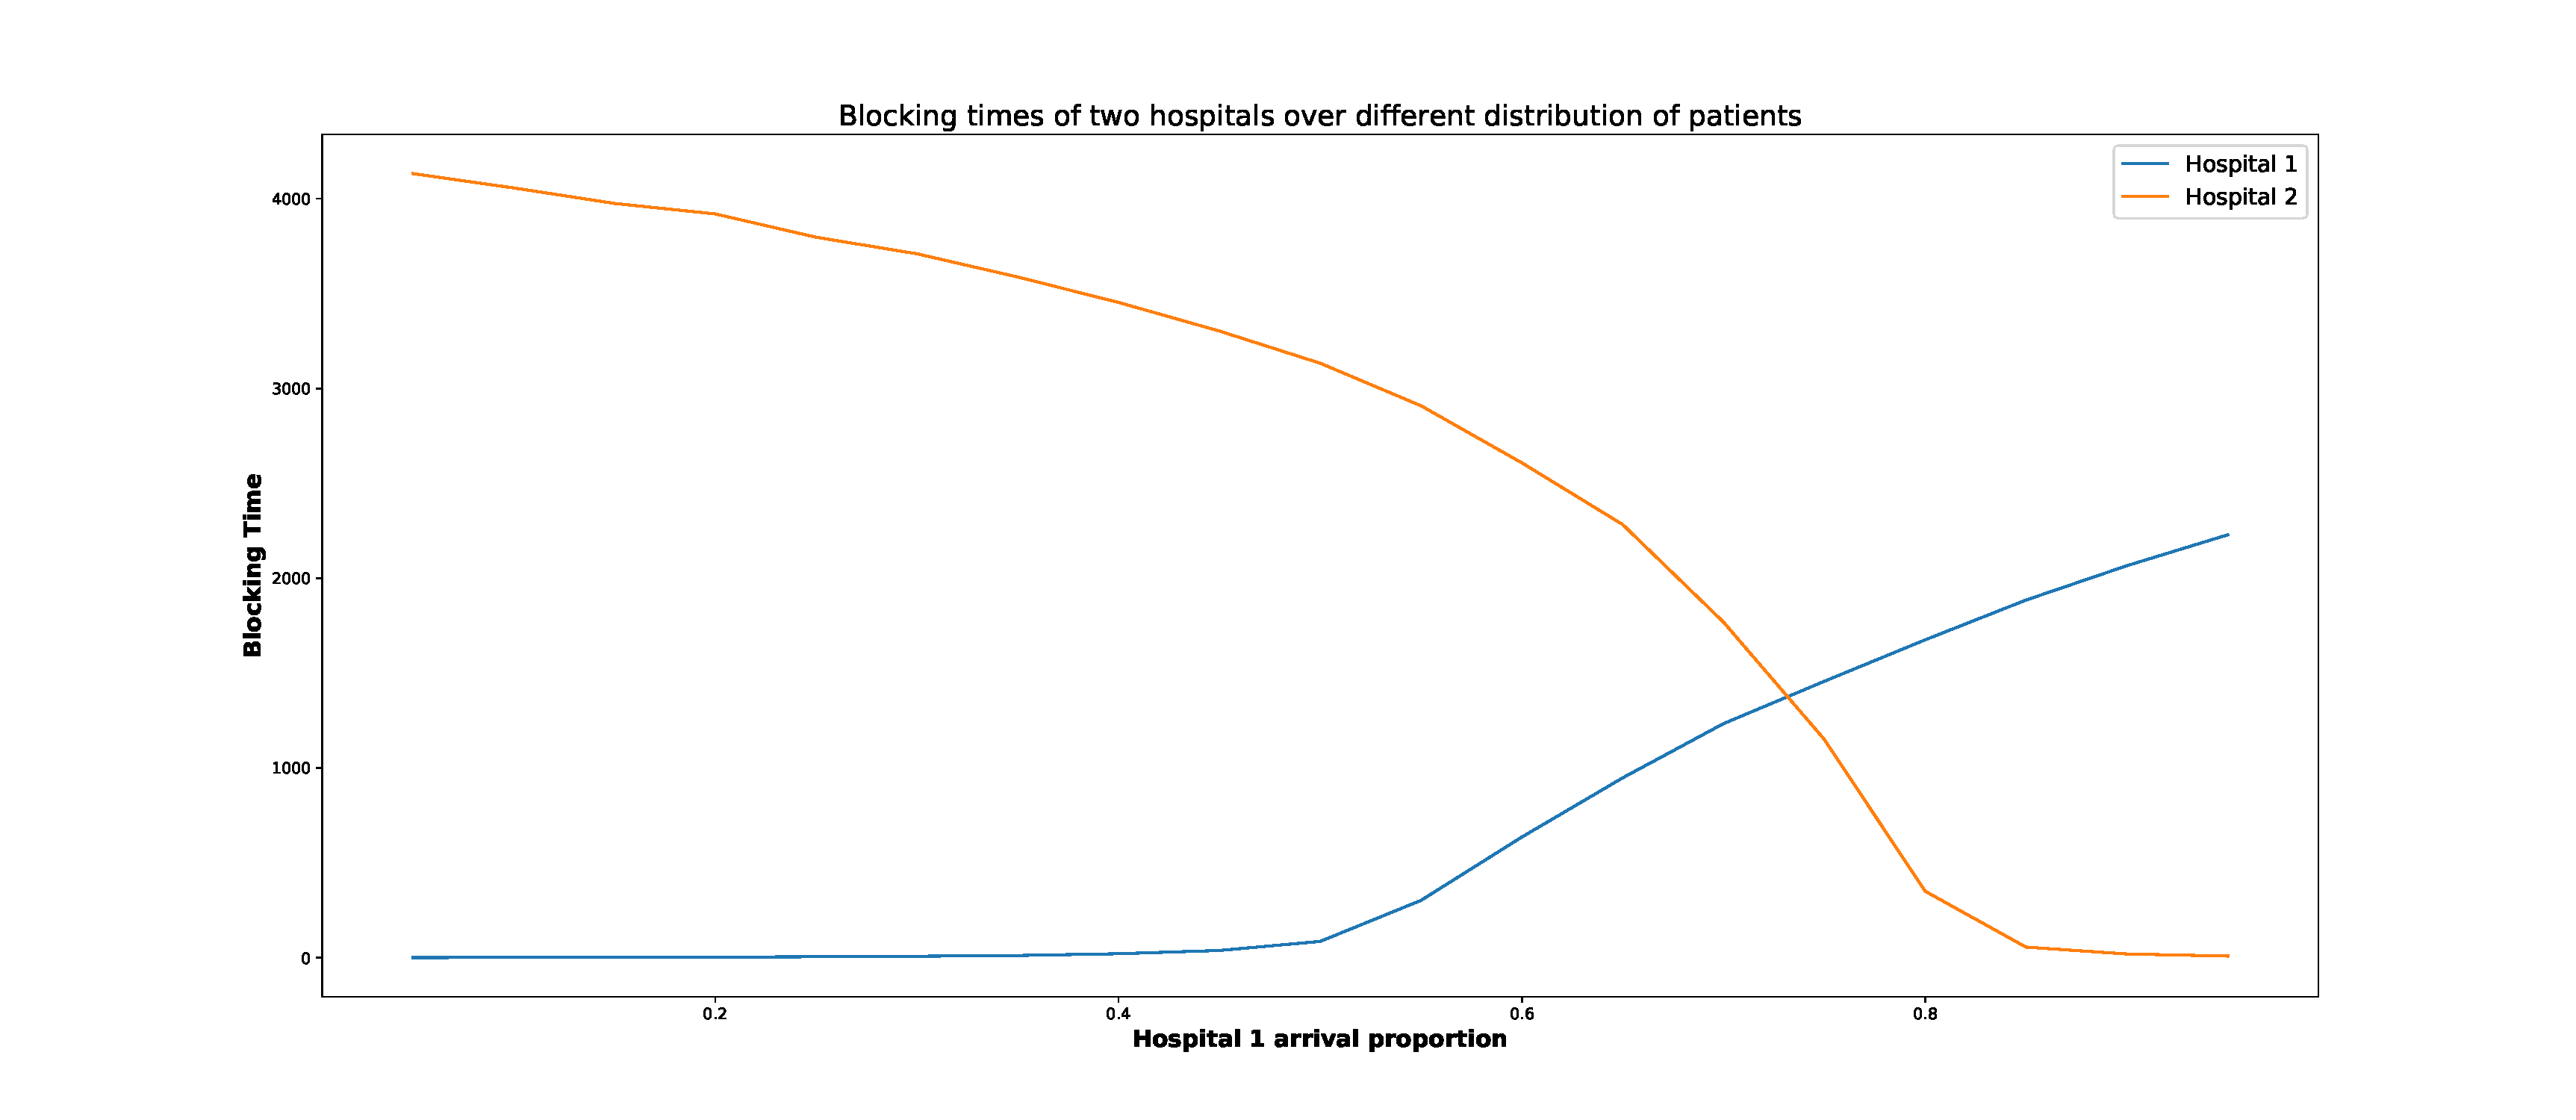
\includegraphics[trim=140 40 150 50, clip, width=\textwidth]{Bin/src/optimal_patient.pdf}

    \begin{equation*}
        B_1 = B_2
    \end{equation*}
\end{frame}


\begin{frame}
    \frametitle{Future Plans}
    \centering
    \begin{tikzpicture}[-, node distance = 3cm, scale=0.8]
        \node[anchor=north](H1){\(H_1\)};
        \node[anchor=north](H1_d1) at (3, 2){.};
        \node[anchor=north](H1_d2) at (3, -2){.};

        \path[->] (H1) edge node {}(H1_d1);
        \path[->] (H1) edge node {}(H1_d2);
        \path (H1_d1) edge [bend left] node {}(H1_d2);
        \path (H1_d1) [dashed] edge node {}(H1_d2);

        \node[anchor=north](H2) at (3.9, 0){\(H_2\)};
        \node[anchor=north](H2_d1) at (6.9, 2){.};
        \node[anchor=north](H2_d2) at (6.9, -2){.};

        \path[->] (H2) edge node {}(H2_d1);
        \path[->] (H2) edge node {}(H2_d2);
        \path(H2_d1) edge [bend left] node {}(H2_d2);

        \node[anchor=north](A) at (7.8, 0){\(A\)};
        \node[anchor=north](A_d1) at (10.8, 2){.};
        \node[anchor=north](A_d2) at (10.8, -2){.};
        
        \path[->] (A) edge node {}(A_d1);
        \path[->] (A) edge node {}(A_d2);
        \path(A_d1) edge [bend left] node {}(A_d2);
    \end{tikzpicture}
\end{frame}